\chapter{Force, Mass, and Acceleration}

\section{Mass and Acceleration}

Each atom has a mass, which means everything made up of those atoms has mass as 
well (and that's pretty much everything!). We measure mass in grams. A paper clip 
is about 1 gram of steel. An adult human can have a mass of 70,000 grams, so for 
larger things, we often talk about kilograms, which is 1000 grams.

The first interesting thing about mass is that objects with more mass
require more force to accelerate. For example, pushing a bicycle so
that it accelerates from a standstill to jogging speed in 2 seconds
requires much less force than pushing a train so that it accelerates
at the same rate.


\begin{mdframed}[style=important, frametitle={Newton's Second Law of Motion}]

The force necessary to accelerate an object of mass $m$ at an acceleration of
$a$ is given by:
$$F = m a$$

This means the force is equal to the mass times the acceleration.

\end{mdframed}

What are the units here? We already know that mass is measured in
kilograms. We can measure velocity in meters per second, but that is
different from acceleration. Acceleration is the rate of change in
velocity. So if we want to go from 0 to 5 meters per second (that's
jogging speed) in two seconds, that is a change in velocity of 2.5
meters per second every second. We would say this acceleration is $2.5
m/s^2$.

\subsection{Velocity versus Acceleration}
Acceleration is the change in velocity. If an object is speeding up or slowing 
down, it is accelerating. In everyday language, we often use \textit{decelerate} 
to indicate slowing down, but in physics you can use the word accelerate (slowing 
down is just negative acceleration). Since velocity is a vector (it has a 
magnitude and direction), changing direction is \textit{also acceleration}. On 
the other hand, an object moving at a constant velocity (same speed, same 
direction) is \textit{not accelerating}!

\begin{Exercise}[title = {Is it accelerating?}, label = accel]
State whether the described object is accelerating or not. 
\begin{enumerate}
\item A satellite orbiting the Earth at a constant speed.
\item A car moving due west at a constant 30 mile per hour.
\item A child coming to a stop on their bicycle.
\item A roller coaster going around a loop at a constant speed.
\item A roller coaster speeding up as it goes down the initial hill.
\item A book sitting on a table. 
\end{enumerate}
\end{Exercise}

\begin{Answer}[ref = accel]
\begin{enumerate}
\item acceleration: the satellite is moving in a circle, therefore changing 
direction and accelerating.
\item Not acceleration: the car isn't changing speed or direction.
\item Acceleration: the child is changing speed.
\item Acceleration: the roller coaster is changing direction.
\item Acceleration: the roller coaster is changing speed. 
\item Not acceleration: the book isn't changing speed or direction.
\end{enumerate}
\end{Answer}

It's a common misconception that all objects in motion are accelerating. If an 
object is moving with a constant velocity (same speed, same direction), then it 
is not accelerating. 

\subsection{Calculating Acceleration}
When an object is speeding up or slowing down, we can calculate the acceleration 
by dividing the change in velocity by the time it takes to make that change. 

\begin{mdframed}[style = important, frametitle = {Calculating Acceleration}]
The acceleration of an object from an initial velocity, $v_i$, to a final
velocity, $v_f$, over a period of time, $t$, is given by:

$$a = \frac{v_f - v_i}{t}$$
\end{mdframed}

Notice that if the velocity does not change, then $v_f - v_i = 0$ and the 
acceleration is also zero.

\textbf{Example}: Your car can go from zero to 60 mph in 3 seconds. What is the
acceleration in $m / s^2$?

\textbf{Solution}: First, let's convert from the imperial units of miles per
hour to the SI units of meters per second. You can do this using a search engine, 
but we will show how to do it by hand below. (You will learn more about this 
method in the Units chapter).

$$\frac{60 \text{ miles}}{1 \text{ hour}} \cdot \frac{1.61 \text{ km}}{1 
\text{ mile}} \cdot \frac{1000\text{ m}}{1\text{ km}} \cdot \frac{1\text{ hour}}{
3600\text{ seconds}} \approx \frac{26.82\text{ m}}{s}$$

Now we have the starting velocity (0 m/s), the ending velocity (26.82 m/s), and 
the time (3 s), and we can find the acceleration:
$$a = \frac{v_f - v_i}{t} = \frac{26.82\frac{m}{s} - 0\frac{m}{s}}{3s} \approx 
8.94 \frac{m}{s^2}$$

\subsection{Determining Force}
What about measuring force? Newton decided to name the unit after himself: The
force necessary to accelerate one kilogram at $1 m/s^2$ is known as \textit{a
newton}. It is often denoted by the symbol $N$.

$$1 N = 1 \frac{kg \cdot m}{s^2}$$

\textbf{Example}: If the car in the above example has a mass of 1500 kg, how much 
force does the engine use to accelerate the car?

\textbf{Solution}: We have already found the car's acceleration: 8.94 $m/s^2$. 
With the mass and acceleration, we can use Newton's Second Law to find the force 
needed to accelerate the car:
$$F = m \cdot a = 1500\text{ kg} \cdot 8.94 \frac{m}{s^2} = 13410\text{ N}$$

\begin{Exercise}[title={Acceleration}, label=acceleration_train]

While driving a bulldozer, you come across a train car (with no brakes
and no locomotive) sitting on a track in the middle of a city. The train car
has a label telling you that it has a mass of 2,400 kg. There is a time-bomb
welded to the interior of the train car, and the timer tells you that
you can safely push the train car for 120 seconds. To get the train
car to where it can explode safely, you need to accelerate it to 20 meters per
second. Fortunately, the track is level and the train car's wheels have
almost no rolling resistance.

With what force, in newtons, do you need to push the train for those 120 seconds?

\end{Exercise}
\begin{Answer}[ref=acceleration_train]
If you accelerate to 20 m/s in 120 s, the acceleration is:
$$a = \frac{v_f - v_i}{t} = \frac{20\text{ m/s} - 0\text{ m/s}}{120\text{ s}} = 
\frac{1}{6} \frac{m}{s^2}$$

To achieve this acceleration, you will need to apply a force of:
$$F = m \cdot a = 2400\text{ kg} \cdot \frac{1}{6} \frac{m}{s^2} = 400\text{ }N$$
\end{Answer}

\section{Net Force}
So far, we've looked at examples where only one force is acting on an object. In 
reality, there are usually multiple forces acting on an object. For example, the 
engine pushes your car forward while friction pulls it backwards. Or your chair 
is pushing up on you while gravity pulls you down. How then can we describe the 
motion of an object if more than one force is acting on it?

We can rearrange Newton's Law:
$$a = \frac{F_{net}}{m}$$

This means that an object's acceleration is directly proportional to the 
\textit{net force} acting on the object and inversely proportional to the object's 
mass. The \textit{net force} is the vector sum of all the forces acting on an 
object\index{net force}. The vector sum just means we have to take the direction of 
the force into account. Usually, up and right are positive while down and left are 
negative. You can see some examples in figure \ref{fig:net_forces}.

\begin{figure}
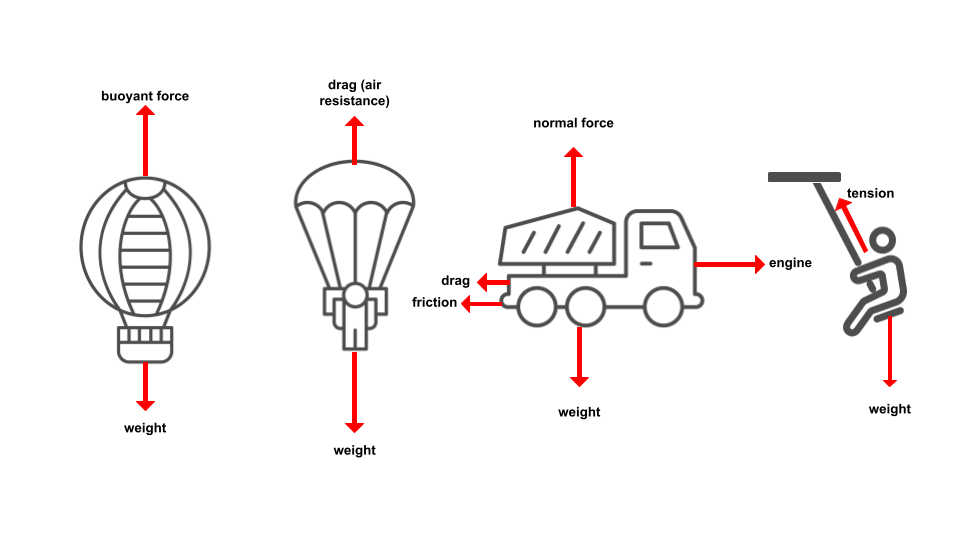
\includegraphics[width=6in]{net_forces.png}
\caption{The hot air balloon has an upwards net force. The parachuter has a downwards net force. The truck has a rightward net force. The swinger has a leftward net force.}
\label{fig:net_forces}
\end{figure}

For now, we'll only look at parallel forces (up/down or left/right). You'll learn 
to use vector addition to combine orthogonal (at right angles) and skew (at angles
other than parallel or right) forces in a later chapter. 

\textbf{Example}: A donkey and a horse are each pulling a cart. The donkey pulls 
to the left with a force of 1500 N, while the horse pulls to the right with a 
force of 2000 N. What is the net force on the cart? If the cart has a mass of 
1000 kg, in what direction and with what magnitude will the cart accelerate?

\textbf{Solution}: We begin by drawing a diagram (this is good practice - while 
a diagram may not be necessary for such a simple question, it will be very useful 
as we examine more complex scenarios in future chapters). 

\begin{center}
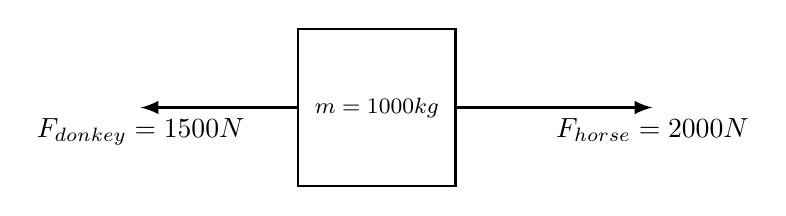
\begin{tikzpicture}
    \draw[thick, black] (-1, -1) rectangle (1,1);
    \draw[very thick, black, -latex] (-1, 0) -- (-3, 0) node[below] {$F_{donkey} 
    = 1500N$};
    \draw[very thick, black, -latex] (1, 0) -- (3.5, 0) node[below] {$F_{horse}=
    2000N$};
    \node[font = \footnotesize] at (0,0) {$m=1000kg$};
\end{tikzpicture}
\end{center}

It is customary to take right as positive, so the horse applies a positive force 
while the donkey applies a negative force to the cart. Therefore, the net force 
is:

$$F_{net} = F_{horse} - F_{donkey} = 2000N - 1500N = 500N$$

Since the net force is positive, it points to the right and the cart will 
accelerate to the right at a rate of:
$$a = \frac{F_{net}}{m} = \frac{500 N}{1000 kg} = 0.5 \frac{m}{s^2}$$

\begin{Exercise}[title = {Net Force and Acceleration}, label = netF]
Rank the acceleration of the boxes shown below from greatest to least. All 
surfaces are frictionless and each box starts at rest. Take left as negative, and 
negative accelerations are less than a zero acceleration.

\begin{tikzpicture}
    \draw[thick, fill=gray!50] (-1.5, 1.5) rectangle (-0.5, 2) node[above, 
    xshift = -0.5cm] {\textbf{A}};
    \node[font = \footnotesize] at (-1, 1.75) {1 kg};
    \draw[pattern = north west lines] (-2, 1.5) rectangle (0, 1.25);
    \draw[very thick, -latex] (-0.5, 1.75) -- (0.5, 1.75) node[above] 
    {$F_1 = 4N$};
    \draw[very thick, -latex] (-1.5, 1.75) -- (-2.25, 1.75) node[above] 
    {$F_2 = 3N$};

    \draw[thick, fill=gray!50] (4, 1.5) rectangle (5, 2) node[above, 
    xshift=-0.5cm] {\textbf{B}};
    \node[font = \footnotesize] at (4.5, 1.75) {1 kg};
    \draw[pattern = north west lines] (3.5, 1.5) rectangle (5.5, 1.25);
    \draw[very thick, -latex] (4, 1.75) -- (3, 1.75) node[above] 
    {$F_2 = 4N$};
    \draw[very thick, -latex] (5, 1.75) -- (5.75, 1.75) node[above] 
    {$F_1 = 3N$};

    \draw[thick, fill=gray!50] (-1.5, -0.5) rectangle (-0.5, 0) node[above, 
    xshift=-0.5cm] {\textbf{C}};
    \node[font = \footnotesize] at (-1, -0.25) {0.5 kg};
    \draw[pattern = north west lines] (-2, -0.5) rectangle (0, -0.75);
    \draw[very thick, -latex] (-0.5, -0.25) -- (0.5, -0.25) node[above] 
    {$F_1 = 4N$};
    \draw[very thick, -latex] (-1.5, -0.25) -- (-2.25, -0.25) node[above] 
    {$F_2 = 3N$};

    \draw[thick, fill=gray!50] (4, -0.5) rectangle (5, 0) node[above, 
    xshift=-0.5cm] {\textbf{D}};
    \node[font = \footnotesize] at (4.5, -0.25) {0.5 kg};
    \draw[pattern = north west lines] (3.5, -0.5) rectangle (5.5, -0.75);
    \draw[very thick, -latex] (4, -0.25) -- (3, -0.25) node[above] {$F_2 = 4N$};
    \draw[very thick, -latex] (5, -0.25) -- (5.75, -0.25) node[above] 
    {$F_1 = 3N$};

    \draw[thick, fill=gray!50] (-1.5, -2.5) rectangle (-0.5, -2) node[above, 
    xshift=-0.5cm] {\textbf{E}};
    \node[font = \footnotesize] at (-1, -2.25) {0.5 kg};
    \draw[pattern = north west lines] (-2, -2.5) rectangle (0, -2.75);
    \draw[very thick, -latex] (-0.5, -2.25) -- (0.75, -2.25) node[above] 
    {$F_1 = 5N$};
    \draw[very thick, -latex] (-1.5, -2.25) -- (-2.75, -2.25) node[above] 
    {$F_2 = 5N$};    

    \draw[thick, fill=gray!50] (4, -2.5) rectangle (5, -2) node[above, 
    xshift=-0.5cm] {\textbf{F}};
    \node[font = \footnotesize] at (4.5, -2.25) {1 kg};
    \draw[pattern = north west lines] (3.5, -2.5) rectangle (5.5, -2.75);
    \draw[very thick, -latex] (4, -2.25) -- (2.75, -2.25) node[above] 
    {$F_2 = 5N$};
    \draw[very thick, -latex] (5, -2.25) -- (6.25, -2.25) node[above] 
    {$F_1 = 5N$};
\end{tikzpicture}
\end{Exercise}

\begin{Answer}[ref = netF]
C, A, E/F, B, D
$$a_A = \frac{F_{net, A}}{m_A} = \frac{4N - 3N}{1kg} = \frac{1N}{1kg} = 1 
\frac{m}{s^2}$$
$$a_B = \frac{F_{net, B}}{m_B} = \frac{3N - 4N}{1kg} = \frac{-1N}{1kg} = -1 
\frac{m}{s^2}$$
$$a_C = \frac{F_{net, C}}{m_C} = \frac{4N - 3N}{0.5kg} = \frac{1N}{0.5kg} = 2 
\frac{m}{s^2}$$
$$a_D = \frac{F_{net, D}}{m_D} = \frac{3N - 4N}{0.5kg} = \frac{-1N}{0.5kg} = -2 
\frac{m}{s^2}$$
$$a_E = \frac{F_{net, E}}{m_E} = \frac{5N - 5N}{0.5kg} = \frac{0N}{0.5kg} = 0 
\frac{m}{s^2}$$
$$a_F = \frac{F_{net, F}}{m_F} = \frac{5N - 5N}{1kg} = \frac{0N}{1kg} = 0 
\frac{m}{s^2}$$
\end{Answer}

\section{Normal Force and Apparent Weight}
If you were to stand on a scale while riding an elevator, you would see the scale 
fluctuate as the elevator accelerates up and down (if you have a bathroom scale 
and live in a building with an elevator, you can try this yourself!). The reading 
on the scale is your \textit{apparent weight} and is equal to the normal force 
between you and the floor. 

What is a \textit{normal force}? First, the word ``normal" doesn't have the 
colloquial meaning of average or usual. In mathematics, ``normal" means 
perpendicular. A normal force is perpendicular to the contact surface between 
two objects. Let's look at a person standing at rest. We know that gravity is 
pulling down on the person:

\begin{center}
    \begin{tikzpicture}
        %\draw[step=1cm, gray, very thin] (-2, -4) grid (2, 0);

        %floor
        \draw[pattern = north west lines] (-4, 0) rectangle (4, -0.5);

        %arrows and labels
        \draw[red, fill=red] (0, -2) -- (0.5, -1.5) -- (0.25, -1.5) -- (0.25, 0.5) -- (-0.25, 0.5) -- (-0.25, -1.5) -- (-0.5, -1.5) -- cycle;
        \node[] at (0, -2.25) {Weight};
        \node[] at (0, -2.75) {$F_g = mg$};
    
        %person fill
        \draw[gray, fill=gray] (-0.5, 0.5) circle (0.5cm);
        \draw[gray, fill=gray] (0.5, 0.5) circle (0.5cm);
        \draw[gray, fill=gray] (-1, 0.5) rectangle (1, 4);
        \draw[gray, fill=gray] (-1.25, 2.5) circle (0.25cm);
        \draw[gray, fill=gray] (1.25, 2.5) circle (0.25cm);
        \draw[gray, fill=gray] (-1.5, 2.5) rectangle (-1, 5);
        \draw[gray, fill=gray] (1, 2.5) rectangle (1.5, 5);
        \draw[gray, fill=gray] (0, 6.25) circle (0.75cm);
        \draw[gray, fill=gray] (-1, 5) circle (0.5cm);
        \draw[gray, fill=gray] (1, 5) circle (0.5cm);
        \draw[gray, fill=gray] (-1, 4) rectangle (1, 5.5);

        %person outline
        \draw[] (-1, 4.5) -- (-1, 0.5) arc (180:360:0.5);
        \draw[] (0, 0.5) arc (180:360:0.5) -- (1,4.5);
        \draw[] (0, 0.5) -- (0,2.75);
        \draw[] (1, 2.5) arc (180:360:0.25) -- (1.5, 5) arc (0:90:.5) -- (-1, 5.5) arc (90:180:0.5) -- (-1.5, 2.5) arc (180:360:0.25);
        \draw[] (0, 6.25) circle (0.75cm);
    \end{tikzpicture}
\end{center}

Since the person is not accelerating, there must be some other force acting on 
them in the upwards direction that balances out the person's weight (recall that 
if $a=0 m/s^2$, then it must be true that $F_{net} = 0N$). In this case, the 
balancing force is the \textit{normal force} of the floor pushing up on the 
person's feet:

\begin{center}
    \begin{tikzpicture}
        %\draw[step=1cm, gray, very thin] (-2, -4) grid (2, 0);

        %floor
        \draw[pattern = north west lines] (-4, 0) rectangle (4, -0.5);

        %down arrows and labels
        \draw[red, fill=red] (-0.5, -2) -- (0, -1.5) -- (-0.25, -1.5) -- (-0.25, 0.5) -- (-0.75, 0.5) -- (-0.75, -1.5) -- (-1, -1.5) -- cycle;
        \node[] at (-0.5, -2.25) {Weight};
        \node[] at (-0.5, -2.75) {$F_g = mg$};
    
        %person fill
        \draw[gray, fill=gray] (-0.5, 0.5) circle (0.5cm);
        \draw[gray, fill=gray] (0.5, 0.5) circle (0.5cm);
        \draw[gray, fill=gray] (-1, 0.5) rectangle (1, 4);
        \draw[gray, fill=gray] (-1.25, 2.5) circle (0.25cm);
        \draw[gray, fill=gray] (1.25, 2.5) circle (0.25cm);
        \draw[gray, fill=gray] (-1.5, 2.5) rectangle (-1, 5);
        \draw[gray, fill=gray] (1, 2.5) rectangle (1.5, 5);
        \draw[gray, fill=gray] (0, 6.25) circle (0.75cm);
        \draw[gray, fill=gray] (-1, 5) circle (0.5cm);
        \draw[gray, fill=gray] (1, 5) circle (0.5cm);
        \draw[gray, fill=gray] (-1, 4) rectangle (1, 5.5);

        %person outline
        \draw[] (-1, 4.5) -- (-1, 0.5) arc (180:360:0.5);
        \draw[] (0, 0.5) arc (180:360:0.5) -- (1,4.5);
        \draw[] (0, 0.5) -- (0,2.75);
        \draw[] (1, 2.5) arc (180:360:0.25) -- (1.5, 5) arc (0:90:.5) -- (-1, 5.5) arc (90:180:0.5) -- (-1.5, 2.5) arc (180:360:0.25);
        \draw[] (0, 6.25) circle (0.75cm);

        %up arrows and labels
         \draw[blue, fill=blue] (0.25, 0) -- (0.25, 1.5) -- (0, 1.5) -- (0.5, 2) -- (1, 1.5) -- (0.75, 1.5) -- (0.75, 0) -- cycle;
         \node[] at (0.5, 2.25) {$F_N$};
         \node[] at (0.5, 2.75) {Normal Force};
    \end{tikzpicture}
\end{center}

%fix me explanation of normal force? intuitive explanation of deformation, atoms being pressed together and repelling, rebound of table. There's a demo where you shine a laser at an angle on a mirror flat on a table, then put weight on the table. students can see that the table deforms and helps students to "justify" where the normal force comes from. didn't find a good youtube video but i'll keep looking

When you step on a bathroom scale, it is actually measuring the normal force! 
When you are not accelerating, your weight and the normal force between you and 
the scale are equal, so the scale gives you an accurate measure of your weight. 
Let's look at what happens if you are accelerating, as in an elevator.

\textbf{Example}: Maria has a mass of 80. kg. If the elevator in her apartment 
building initially accelerates at 0.50 $m/s^2$, what is her apparent weight as 
the elevator begins to move down?

\textbf{Solution}: We begin with a diagram:
\begin{center}
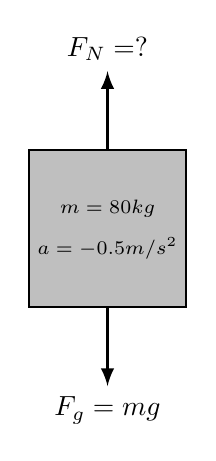
\begin{tikzpicture}
	\draw[thick, fill = gray!50] (-1, -1) rectangle (1, 1);
	\node[font = \scriptsize] at (0,0.25) {$m=80kg$};
	\node[font = \scriptsize] at (0, -0.25) {$a=-0.5m/s^2$};
	\draw[very thick, -latex] (0, -1) -- (0, -2) node[below] {$F_g = mg$};
	\draw[very thick, -latex] (0, 1) -- (0, 2) node[above] {$F_N = ?$};
\end{tikzpicture}
\end{center}

Her apparent weight is the normal force. Seeing that the net force acting on 
Maria is given by $F_N - F_g$, we can use Newton's Second Law to find $F_N$:

$$F_{net} = F_N - F_g = ma$$
$$F_N - \left( 80 kg \right) \left(9.8 \frac{m}{s^2} \right) = \left( 80 kg 
\right) \left( -0.5 \frac{m}{s^2} \right)$$
$$F_N = \left( 80 kg \right) \left( 9.8 \frac{m}{s^2} - 0.5 \frac{m}{s^2} 
\right) = 744 N$$

Maria's apparent weight is 744 newtons when the elevator is accelerating 
downwards. 

\begin{Exercise}[title = Moving Elevators, label = elevator]
A 700-N person is standing on a scale in an elevator. Rank the reading on the 
scale from greatest to least for the following scenarios:
\begin{enumerate}
\item The elevator has an initial upward velocity of 2 m/s and an upward 
acceleration of 3 $m/s^2$
\item The elevator is initially at rest and has an upward acceleration of 3 
$m/s^2$
\item The elevator has an initial downward velocity of 2 m/s and an upward 
acceleration of 5 $m/s^2$
\item The elevator is initially at rest and has a downward acceleration of 
9.8 $m/s^2$
\item The elevator has an initial upward velocity of 2 m/s and a downward 
acceleration of 5 $m/s^2$
\item The elevator has an initial downward velocity of 2 m/s and is not 
accelerating 
\end{enumerate}
\end{Exercise}

\begin{Answer}[ref = elevator]
3, 1/2, 6, 5, 4
The velocity does not affect the apparent weight, only the acceleration. If the 
elevator is accelerating upwards, the apparent weight increases. If the elevator 
is accelerating downwards, the apparent weight decreases. In fact, for scenario 
4, the elevator is in free-fall and the person has no apparent weight. When the 
elevator is not accelerating, the person's apparent weight is their true weight. 
\end{Answer}

\subsection{The Normal Force on Slopes}
%normal force is perpendicular to surface, example, exercise draw direction of normal force vector for various things at angles, or leaning against a wall, etc.

\section{Newtons and Joules}
You now know the fundamental units for newtons and joules, which hints at the 
relationship between force and energy:
$$N = \frac{kg \cdot m}{s^2} \text{     } J = \frac{kg \cdot m^2}{s^2} = N \cdot m$$

A joule is equivalent to a newton times a meter. So, multiplying a force 
(newtons) by a displacement (meters) tells you how the energy (joules) of the 
object changes. This relationship is described by the Work-Kinetic Energy Theorem, 
which we will explore in the next chapter. 
